\appendix
\section{Technical appendix}
\label{sec:appendix}

\subsection{The complete lists of used characters relfecting both form and function across case studies}
\subsubsection{Barcelona}

The data for the Barcelona case study has been retrieved from the Barcelona's City Hall
Open Data Service Open Data BCN available at
\href{https://opendata-ajuntament.barcelona.cat}{opendata-ajuntament.barcelona.cat},
\href{https://osm.org}{OpenStreetMap}, and Spanish Cadastre available at
\href{https://catastro.minhap.es}{catastro.minhap.es}. The data represents versions
available on December 01, 2020.

\small
\begin{longtable}{p{5cm}p{4cm}p{4cm}l}
\caption{The complete list of form characters used in the Barcelona case study. The implementation details are available
in Jupyter notebooks available at <anonymised for peer-review>.}
\label{tab:form_bcn} \\
\toprule
                                   index &                         element &                    context &     category \\
\midrule
\endfirsthead

\toprule
                               index &                         element &                    context &     category \\
\midrule
\endhead
\midrule
\multicolumn{4}{r}{{Continued on next page}} \\
\midrule
\endfoot

\bottomrule
\endlastfoot
                                area &                        building &                   building &    dimension \\
                           perimeter &                        building &                   building &    dimension \\
                      courtyard area &                        building &                   building &    dimension \\
                circular compactness &                        building &                   building &        shape \\
                             corners &                        building &                   building &        shape \\
                          squareness &                        building &                   building &        shape \\
        equivalent rectangular index &                        building &                   building &        shape \\
                          elongation &                        building &                   building &        shape \\
centroid - corner distance deviation &                        building &                   building &        shape \\
     centroid - corner mean distance &                        building &                   building &    dimension \\
                   solar orientation &                        building &                   building & distribution \\
                    street alignment &                        building &                   building & distribution \\
                      cell alignment &                        building &                   building & distribution \\
                 longest axis length &               tessellation cell &          tessellation cell &    dimension \\
                                area &               tessellation cell &          tessellation cell &    dimension \\
                circular compactness &               tessellation cell &          tessellation cell &        shape \\
        equivalent rectangular index &               tessellation cell &          tessellation cell &        shape \\
                   solar orientation &               tessellation cell &          tessellation cell & distribution \\
                 coverage area ratio &               tessellation cell &          tessellation cell &    intensity \\
                    street alignment &               tessellation cell &          tessellation cell & distribution \\
                              length &                  street segment &             street segment &    dimension \\
                               width &                  street profile &             street segment &    dimension \\
                            openness &                  street profile &             street segment & distribution \\
                     width deviation &                  street profile &             street segment &    diversity \\
                           linearity &                  street segment &             street segment &        shape \\
                        area covered &                  street segment &             street segment &    dimension \\
                 buildings per meter &                  street segment &             street segment &    intensity \\
                        area covered &                     street node &                street node &    dimension \\
                           alignment &          neighbouring buildings & neighbouring cells (queen) & distribution \\
                       mean distance &          neighbouring buildings & neighbouring cells (queen) & distribution \\
                 weighted neighbours &               tessellation cell & neighbouring cells (queen) & distribution \\
                        area covered &              neighbouring cells & neighbouring cells (queen) &    dimension \\
                        reached area &           neighbouring segments &      neighbouring segments &    dimension \\
                       reached cells &           neighbouring segments &      neighbouring segments &    intensity \\
                              degree &                     street node &         neighbouring nodes & distribution \\
 mean distance to neighbouring nodes &                     street node &         neighbouring nodes &    dimension \\
                  shared walls ratio &             adjacent buildings  &        adjacent buildings  & distribution \\
        mean inter-building distance &          neighbouring buildings &    cell queen neighbours 3 & distribution \\
         weighted reached enclosures & neighbouring tessellation cells &    cell queen neighbours 3 &    intensity \\
                                area &                       enclosure &                  enclosure &    dimension \\
                           perimeter &                       enclosure &                  enclosure &    dimension \\
                circular compactness &                       enclosure &                  enclosure &        shape \\
        equivalent rectangular index &                       enclosure &                  enclosure &        shape \\
           compactness-weighted axis &                       enclosure &                  enclosure &        shape \\
                   solar orientation &                       enclosure &                  enclosure & distribution \\
                 weighted neighbours &                       enclosure &                  enclosure & distribution \\
                      weighted cells &                       enclosure &                  enclosure &    intensity \\
                    local meshedness &                  street network &              nodes 5 steps & connectivity \\
                 mean segment length &                  street network &            segment 3 steps &    dimension \\
                   cul-de-sac length &                  street network &              nodes 3 steps &    dimension \\
                        node density &                  street network &              nodes 5 steps &    intensity \\
           proportion of cul-de-sacs &                  street network &              nodes 5 steps & connectivity \\
   proportion of 3-way intersections &                  street network &              nodes 5 steps & connectivity \\
   proportion of 4-way intersections &                  street network &              nodes 5 steps & connectivity \\
        degree weighted node density &                  street network &              nodes 5 steps &    intensity \\
          local closeness centrality &                  street network &              nodes 5 steps & connectivity \\
               perimeter wall length &             adjacent buildings  &           joined buildings &    dimension \\
                number of courtyards &             adjacent buildings  &           joined buildings &    intensity \\
                   square clustering &                  street network &             street network & connectivity \\
\end{longtable}


\begin{longtable}{p{5cm}p{3cm}p{5cm}}
\caption{The complete list of function characters and transfer methods used in the Barcelona case study. The implementation details are available
in Jupyter notebooks available at <anonymised for peer-review>.}
\label{tab:fn_bcn} \\
\toprule
                                         character & input spatial unit &                                    transfer method \\
\midrule
\endfirsthead

\toprule
                                         character & input spatial unit &                                    transfer method \\
\midrule
\endhead
\midrule
\multicolumn{3}{r}{{Continued on next page}} \\
\midrule
\endfoot

\bottomrule
\endlastfoot
                                        population &              block &                  Building-based Dasymetric mapping \\
                               number of car parks &              block &                                 Dasymetric mapping \\
       number of other items that are not premises &              block &                                 Dasymetric mapping \\
                                          land use &             parcel &                            Spatial join (centroid) \\
                               number of dwellings &           building &                                     Attribute join \\
                                       current use &           building &                                     Attribute join \\
                                               age &           building &                                     Attribute join \\
                                          heritage &             points &                     Accessibility  -\# within 15min \\
                                          heritage &           polygons &                                       Spatial join \\
   culture (cinemas, museums, libraries, theaters) &             points & Accessibility  - distance to nearest / \# within 15min \\
                                             parks &             points & Accessibility  - distance to nearest / \# within 15min \\
                                   economic census &            poitnts & Accessibility  - distance to nearest / \# within 15min \\
                                       restaurants &              point & Accessibility  - distance to nearest / \# within 15min \\
                                             trees &             points &                               Spatial join (count) \\
                                              NDVI &          raster 1m &                                        Zonal stats \\
\end{longtable}

\subsubsection{Medellin}

The data for the Medellin case study has been retrieved from the GeoMedellin Open Data
 portal available at
 \href{https://www.medellin.gov.co/geomedellin/}{medellin.gov.co/geomedellin/},
 \href{https://osm.org}{OpenStreetMap}, WorldPop gridded population estimates
 \citep{bondarenko2020census}, and a Sentinel 2 cloud-free composite
 \citep{CORBANE2020105737}. The data represents versions available on January 05, 2021.

\begin{longtable}{p{5cm}p{4cm}p{4cm}l}
\caption{The complete list of form characters used in the Medellin case study. The implementation details are available
in Jupyter notebooks available at <anonymised for peer-review>.}
\label{tab:form_med} \\
\toprule
                                index &                         element &                    context &     category \\
\midrule
\endfirsthead

\toprule
                                index &                         element &                    context &     category \\
\midrule
\endhead
\midrule
\multicolumn{4}{r}{{Continued on next page}} \\
\midrule
\endfoot

\bottomrule
\endlastfoot
                                area &                        building &                   building &    dimension \\
                            perimeter &                        building &                   building &    dimension \\
                        courtyard area &                        building &                   building &    dimension \\
                circular compactness &                        building &                   building &        shape \\
                                corners &                        building &                   building &        shape \\
                            squareness &                        building &                   building &        shape \\
        equivalent rectangular index &                        building &                   building &        shape \\
                            elongation &                        building &                   building &        shape \\
centroid - corner distance deviation &                        building &                   building &        shape \\
        centroid - corner mean distance &                        building &                   building &    dimension \\
                    solar orientation &                        building &                   building & distribution \\
                    street alignment &                        building &                   building & distribution \\
                        cell alignment &                        building &                   building & distribution \\
                    longest axis length &               tessellation cell &          tessellation cell &    dimension \\
                                area &               tessellation cell &          tessellation cell &    dimension \\
                circular compactness &               tessellation cell &          tessellation cell &        shape \\
        equivalent rectangular index &               tessellation cell &          tessellation cell &        shape \\
                    solar orientation &               tessellation cell &          tessellation cell & distribution \\
                    coverage area ratio &               tessellation cell &          tessellation cell &    intensity \\
                    street alignment &               tessellation cell &          tessellation cell & distribution \\
                                length &                  street segment &             street segment &    dimension \\
                                width &                  street profile &             street segment &    dimension \\
                            openness &                  street profile &             street segment & distribution \\
                        width deviation &                  street profile &             street segment &    diversity \\
                            linearity &                  street segment &             street segment &        shape \\
                        area covered &                  street segment &             street segment &    dimension \\
                    buildings per meter &                  street segment &             street segment &    intensity \\
                        area covered &                     street node &                street node &    dimension \\
                            alignment &          neighbouring buildings & neighbouring cells (queen) & distribution \\
                        mean distance &          neighbouring buildings & neighbouring cells (queen) & distribution \\
                    weighted neighbours &               tessellation cell & neighbouring cells (queen) & distribution \\
                        area covered &              neighbouring cells & neighbouring cells (queen) &    dimension \\
                        reached area &           neighbouring segments &      neighbouring segments &    dimension \\
                        reached cells &           neighbouring segments &      neighbouring segments &    intensity \\
                                degree &                     street node &         neighbouring nodes & distribution \\
    mean distance to neighbouring nodes &                     street node &         neighbouring nodes &    dimension \\
                    shared walls ratio &             adjacent buildings  &        adjacent buildings  & distribution \\
        mean inter-building distance &          neighbouring buildings &    cell queen neighbours 3 & distribution \\
            weighted reached enclosures & neighbouring tessellation cells &    cell queen neighbours 3 &    intensity \\
                                area &                       enclosure &                  enclosure &    dimension \\
                            perimeter &                       enclosure &                  enclosure &    dimension \\
                circular compactness &                       enclosure &                  enclosure &        shape \\
        equivalent rectangular index &                       enclosure &                  enclosure &        shape \\
            compactness-weighted axis &                       enclosure &                  enclosure &        shape \\
                    solar orientation &                       enclosure &                  enclosure & distribution \\
                    weighted neighbours &                       enclosure &                  enclosure & distribution \\
                        weighted cells &                       enclosure &                  enclosure &    intensity \\
                    local meshedness &                  street network &              nodes 5 steps & connectivity \\
                    mean segment length &                  street network &            segment 3 steps &    dimension \\
                    cul-de-sac length &                  street network &              nodes 3 steps &    dimension \\
                        node density &                  street network &              nodes 5 steps &    intensity \\
            proportion of cul-de-sacs &                  street network &              nodes 5 steps & connectivity \\
    proportion of 3-way intersections &                  street network &              nodes 5 steps & connectivity \\
    proportion of 4-way intersections &                  street network &              nodes 5 steps & connectivity \\
        degree weighted node density &                  street network &              nodes 5 steps &    intensity \\
            local closeness centrality &                  street network &              nodes 5 steps & connectivity \\
                perimeter wall length &             adjacent buildings  &           joined buildings &    dimension \\
                number of courtyards &             adjacent buildings  &           joined buildings &    intensity \\
                    square clustering &                  street network &             street network & connectivity \\
\end{longtable}


\begin{longtable}{p{5cm}p{3cm}p{5cm}}
\caption{The complete list of function characters and transfer methods used in the Medellin case study. The implementation details are available
in Jupyter notebooks available at <anonymised for peer-review>.}
\label{tab:fn_med} \\
\toprule
                                            character & input spatial unit &                                    transfer method \\
\midrule
\endfirsthead

\toprule
                                            character & input spatial unit &                                    transfer method \\
\midrule
\endhead
\midrule
\multicolumn{3}{r}{{Continued on next page}} \\
\midrule
\endfoot

\bottomrule
\endlastfoot
                trees &   points &                               Spatial join (count) \\
                parks & polygons &                                Distance to nearest \\
heritage large areas & polygons &                               Spatial join (boolean) \\
            land use & polygons &                                             tobler \\
                pois &   points & Accessibility  - distance to nearest / \# within 15min \\
        public spaces & polygons &             Accessibility  -  area within radius \\
            population &   raster &                                        Zonal stats \\
                NDVI &   raster &                                        Zonal stats \\
\end{longtable}

\subsubsection{Dar es Salaam}

The data for the Dar es Salaam case study has been retrieved from
\href{https://osm.org}{OpenStreetMap}, WorldPop gridded population estimates
\citep{bondarenko2020census}, a Copernicus Global Land Cover
\citep{marcel_buchhorn_2020_3939050}, VIIRS Night lights data (June 2020) \citep{elvidge2013viirs},
and a Sentinel 2 cloud-free composite \citep{CORBANE2020105737}. The data represents
versions available on December 18, 2020.

\begin{longtable}{p{5cm}p{4cm}p{4cm}l}
    \caption{The complete list of form characters used in the Dar es Salaam case study. The implementation details are available
    in Jupyter notebooks available at <anonymised for peer-review>.}
    \label{tab:form_des} \\
    \toprule
                                   index &                         element &                    context &     category \\
    \midrule
    \endfirsthead

    \toprule
                                   index &                         element &                    context &     category \\
    \midrule
    \endhead
    \midrule
    \multicolumn{4}{r}{{Continued on next page}} \\
    \midrule
    \endfoot

    \bottomrule
    \endlastfoot
                                    area &                        building &                   building &    dimension \\
                               perimeter &                        building &                   building &    dimension \\
                          courtyard area &                        building &                   building &    dimension \\
                    circular compactness &                        building &                   building &        shape \\
                                 corners &                        building &                   building &        shape \\
                              squareness &                        building &                   building &        shape \\
            equivalent rectangular index &                        building &                   building &        shape \\
                              elongation &                        building &                   building &        shape \\
    centroid - corner distance deviation &                        building &                   building &        shape \\
         centroid - corner mean distance &                        building &                   building &    dimension \\
                       solar orientation &                        building &                   building & distribution \\
                        street alignment &                        building &                   building & distribution \\
                          cell alignment &                        building &                   building & distribution \\
                     longest axis length &               tessellation cell &          tessellation cell &    dimension \\
                                    area &               tessellation cell &          tessellation cell &    dimension \\
                    circular compactness &               tessellation cell &          tessellation cell &        shape \\
            equivalent rectangular index &               tessellation cell &          tessellation cell &        shape \\
                       solar orientation &               tessellation cell &          tessellation cell & distribution \\
                     coverage area ratio &               tessellation cell &          tessellation cell &    intensity \\
                                  length &                  street segment &             street segment &    dimension \\
                                   width &                  street profile &             street segment &    dimension \\
                                openness &                  street profile &             street segment & distribution \\
                         width deviation &                  street profile &             street segment &    diversity \\
                               linearity &                  street segment &             street segment &        shape \\
                            area covered &                  street segment &             street segment &    dimension \\
                     buildings per meter &                  street segment &             street segment &    intensity \\
                            area covered &                     street node &                street node &    dimension \\
                               alignment &          neighbouring buildings & neighbouring cells (queen) & distribution \\
                           mean distance &          neighbouring buildings & neighbouring cells (queen) & distribution \\
                     weighted neighbours &               tessellation cell & neighbouring cells (queen) & distribution \\
                            area covered &              neighbouring cells & neighbouring cells (queen) &    dimension \\
                           reached cells &           neighbouring segments &      neighbouring segments &    intensity \\
                            reached area &           neighbouring segments &      neighbouring segments &    dimension \\
                                  degree &                     street node &         neighbouring nodes & distribution \\
     mean distance to neighbouring nodes &                     street node &         neighbouring nodes &    dimension \\
            mean inter-building distance &          neighbouring buildings &    cell queen neighbours 3 & distribution \\
             weighted reached enclosures & neighbouring tessellation cells &    cell queen neighbours 3 &    intensity \\
                       reached neighbors & neighbouring tessellation cells &    cell queen neighbours 3 &    intensity \\
                            reached area & neighbouring tessellation cells &    cell queen neighbours 3 &    dimension \\
                                    area &                       enclosure &                  enclosure &    dimension \\
                               perimeter &                       enclosure &                  enclosure &    dimension \\
                    circular compactness &                       enclosure &                  enclosure &        shape \\
            equivalent rectangular index &                       enclosure &                  enclosure &        shape \\
               compactness-weighted axis &                       enclosure &                  enclosure &        shape \\
                       solar orientation &                       enclosure &                  enclosure & distribution \\
                     weighted neighbours &                       enclosure &                  enclosure & distribution \\
                          weighted cells &                       enclosure &                  enclosure &    intensity \\
                        local meshedness &                  street network &              nodes 5 steps & connectivity \\
                     mean segment length &                  street network &            segment 3 steps &    dimension \\
                       cul-de-sac length &                  street network &              nodes 3 steps &    dimension \\
                            reached area &                  street network &            segment 3 steps &    dimension \\
                           reached cells &                  street network &            segment 3 steps &    intensity \\
                            node density &                  street network &              nodes 5 steps &    intensity \\
               proportion of cul-de-sacs &                  street network &              nodes 5 steps & connectivity \\
       proportion of 3-way intersections &                  street network &              nodes 5 steps & connectivity \\
       proportion of 4-way intersections &                  street network &              nodes 5 steps & connectivity \\
            degree weighted node density &                  street network &              nodes 5 steps &    intensity \\
              local closeness centrality &                  street network &              nodes 5 steps & connectivity \\
                       square clustering &                  street network &             street network & connectivity \\
\end{longtable}


\begin{longtable}{p{5cm}p{3cm}p{5cm}}
    \caption{The complete list of function characters and transfer methods used in the Dar es Salaam case study. The implementation details are available
    in Jupyter notebooks available at <anonymised for peer-review>.}
    \label{tab:fn_des} \\
    \toprule
                                             character & input spatial unit &                                    transfer method \\
    \midrule
    \endfirsthead

    \toprule
                                             character & input spatial unit &                                    transfer method \\
    \midrule
    \endhead
    \midrule
    \multicolumn{3}{r}{{Continued on next page}} \\
    \midrule
    \endfoot

    \bottomrule
    \endlastfoot
    population & raster 100m &     Zonal stats \\
          NDVI &  raster 10m &     Zonal stats \\
    land cover &      raster &     Zonal stats \\
  night lights &      raster &     Zonal stats \\
\end{longtable}

\subsubsection{Houston}

The data for the Houston case study has been retrieved from
\href{https://osm.org}{OpenStreetMap}, Microsoft Building Footprints available from
\href{https://www.microsoft.com/en-us/maps/building-footprints}{microsoft.com/en-us/maps/building-footprints},
WorldPop gridded population estimates
\citep{bondarenko2020census}, a Copernicus Global Land Cover
\citep{marcel_buchhorn_2020_3939050}, VIIRS Night lights data (November 2019) \citep{elvidge2013viirs}, a Sentinel 2 cloud-free composite \citep{CORBANE2020105737}, and
the Longitudinal Employer-Household Dynamics data from US Census 2011 available from
\href{https://lehd.ces.census.gov/data/}{lehd.ces.census.gov/data/}. The data represents
versions available on January 13, 2021.

\begin{longtable}{p{5cm}p{4cm}p{4cm}l}
    \caption{The complete list of form characters used in the Houston case study. The implementation details are available
    in Jupyter notebooks available at <anonymised for peer-review>.}
    \label{tab:form_hou} \\
    \toprule
                                   index &                         element &                    context &     category \\
    \midrule
    \endfirsthead

    \toprule
                                   index &                         element &                    context &     category \\
    \midrule
    \endhead
    \midrule
    \multicolumn{4}{r}{{Continued on next page}} \\
    \midrule
    \endfoot

    \bottomrule
    \endlastfoot
                                    area &                        building &                   building &    dimension \\
                               perimeter &                        building &                   building &    dimension \\
                          courtyard area &                        building &                   building &    dimension \\
                    circular compactness &                        building &                   building &        shape \\
                                 corners &                        building &                   building &        shape \\
                              squareness &                        building &                   building &        shape \\
            equivalent rectangular index &                        building &                   building &        shape \\
                              elongation &                        building &                   building &        shape \\
    centroid - corner distance deviation &                        building &                   building &        shape \\
         centroid - corner mean distance &                        building &                   building &    dimension \\
                       solar orientation &                        building &                   building & distribution \\
                        street alignment &                        building &                   building & distribution \\
                          cell alignment &                        building &                   building & distribution \\
                     longest axis length &               tessellation cell &          tessellation cell &    dimension \\
                                    area &               tessellation cell &          tessellation cell &    dimension \\
                    circular compactness &               tessellation cell &          tessellation cell &        shape \\
            equivalent rectangular index &               tessellation cell &          tessellation cell &        shape \\
                       solar orientation &               tessellation cell &          tessellation cell & distribution \\
                     coverage area ratio &               tessellation cell &          tessellation cell &    intensity \\
                                  length &                  street segment &             street segment &    dimension \\
                                   width &                  street profile &             street segment &    dimension \\
                                openness &                  street profile &             street segment & distribution \\
                         width deviation &                  street profile &             street segment &    diversity \\
                               linearity &                  street segment &             street segment &        shape \\
                            area covered &                  street segment &             street segment &    dimension \\
                     buildings per meter &                  street segment &             street segment &    intensity \\
                               alignment &          neighbouring buildings & neighbouring cells (queen) & distribution \\
                           mean distance &          neighbouring buildings & neighbouring cells (queen) & distribution \\
                     weighted neighbours &               tessellation cell & neighbouring cells (queen) & distribution \\
                            area covered &              neighbouring cells & neighbouring cells (queen) &    dimension \\
                           reached cells &           neighbouring segments &      neighbouring segments &    intensity \\
                            reached area &           neighbouring segments &      neighbouring segments &    dimension \\
                                  degree &                     street node &         neighbouring nodes & distribution \\
     mean distance to neighbouring nodes &                     street node &         neighbouring nodes &    dimension \\
            mean inter-building distance &          neighbouring buildings &    cell queen neighbours 3 & distribution \\
             weighted reached enclosures & neighbouring tessellation cells &    cell queen neighbours 3 &    intensity \\
                       reached neighbors & neighbouring tessellation cells &    cell queen neighbours 3 &    intensity \\
                            reached area & neighbouring tessellation cells &    cell queen neighbours 3 &    dimension \\
                                    area &                       enclosure &                  enclosure &    dimension \\
                               perimeter &                       enclosure &                  enclosure &    dimension \\
                    circular compactness &                       enclosure &                  enclosure &        shape \\
            equivalent rectangular index &                       enclosure &                  enclosure &        shape \\
               compactness-weighted axis &                       enclosure &                  enclosure &        shape \\
                       solar orientation &                       enclosure &                  enclosure & distribution \\
                     weighted neighbours &                       enclosure &                  enclosure & distribution \\
                          weighted cells &                       enclosure &                  enclosure &    intensity \\
                        local meshedness &                  street network &              nodes 5 steps & connectivity \\
                     mean segment length &                  street network &            segment 3 steps &    dimension \\
                       cul-de-sac length &                  street network &              nodes 3 steps &    dimension \\
                            reached area &                  street network &            segment 3 steps &    dimension \\
                           reached cells &                  street network &            segment 3 steps &    intensity \\
                            node density &                  street network &              nodes 5 steps &    intensity \\
               proportion of cul-de-sacs &                  street network &              nodes 5 steps & connectivity \\
       proportion of 3-way intersections &                  street network &              nodes 5 steps & connectivity \\
       proportion of 4-way intersections &                  street network &              nodes 5 steps & connectivity \\
            degree weighted node density &                  street network &              nodes 5 steps &    intensity \\
              local closeness centrality &                  street network &              nodes 5 steps & connectivity \\
                       square clustering &                  street network &             street network & connectivity \\
\end{longtable}

\begin{longtable}{p{5cm}p{3cm}p{5cm}}
    \caption{The complete list of function characters and transfer methods used in the Houston case study. The implementation details are available
    in Jupyter notebooks available at <anonymised for peer-review>.}
    \label{tab:fn_hou} \\
    \toprule
                                             character & input spatial unit &                                    transfer method \\
    \midrule
    \endfirsthead

    \toprule
                                             character & input spatial unit &                                    transfer method \\
    \midrule
    \endhead
    \midrule
    \multicolumn{3}{r}{{Continued on next page}} \\
    \midrule
    \endfoot

    \bottomrule
    \endlastfoot
    population &  raster 100m &              Zonal stats \\
          NDVI &   raster 10m &              Zonal stats \\
    land cover &       raster &              Zonal stats \\
  night lights &       raster &              Zonal stats \\
    employment & census block & Dasymetric interpolation \\
historical sites &        point &            Accessibility \\
\end{longtable}

\subsubsection{Singapore}
The data for the Singapore case study has been retrieved from
\href{https://osm.org}{OpenStreetMap}, Singapore Open data portal available at
\href{https://data.gov.sg/}{data.gov.sg}, WorldPop gridded population estimates
\citep{bondarenko2020census}, VIIRS Night lights data (November 2019) \citep{elvidge2013viirs},
and a Sentinel 2 cloud-free composite \citep{CORBANE2020105737}. The data represents
versions available on February 1, 2021.


\begin{longtable}{p{5cm}p{4cm}p{4cm}l}
    \caption{The complete list of form characters used in the Singapore case study. The implementation details are available
    in Jupyter notebooks available at <anonymised for peer-review>.}
    \label{tab:form_sin} \\
    \toprule
                                   index &                         element &                    context &     category \\
    \midrule
    \endfirsthead

    \toprule
                                   index &                         element &                    context &     category \\
    \midrule
    \endhead
    \midrule
    \multicolumn{4}{r}{{Continued on next page}} \\
    \midrule
    \endfoot

    \bottomrule
    \endlastfoot
                                    area &                        building &                   building &    dimension \\
                               perimeter &                        building &                   building &    dimension \\
                          courtyard area &                        building &                   building &    dimension \\
                    circular compactness &                        building &                   building &        shape \\
                                 corners &                        building &                   building &        shape \\
                              squareness &                        building &                   building &        shape \\
            equivalent rectangular index &                        building &                   building &        shape \\
                              elongation &                        building &                   building &        shape \\
    centroid - corner distance deviation &                        building &                   building &        shape \\
         centroid - corner mean distance &                        building &                   building &    dimension \\
                       solar orientation &                        building &                   building & distribution \\
                        street alignment &                        building &                   building & distribution \\
                          cell alignment &                        building &                   building & distribution \\
                     longest axis length &               tessellation cell &          tessellation cell &    dimension \\
                                    area &               tessellation cell &          tessellation cell &    dimension \\
                    circular compactness &               tessellation cell &          tessellation cell &        shape \\
            equivalent rectangular index &               tessellation cell &          tessellation cell &        shape \\
                       solar orientation &               tessellation cell &          tessellation cell & distribution \\
                     coverage area ratio &               tessellation cell &          tessellation cell &    intensity \\
                        street alignment &               tessellation cell &          tessellation cell & distribution \\
                                  length &                  street segment &             street segment &    dimension \\
                                   width &                  street profile &             street segment &    dimension \\
                                openness &                  street profile &             street segment & distribution \\
                         width deviation &                  street profile &             street segment &    diversity \\
                               linearity &                  street segment &             street segment &        shape \\
                            area covered &                  street segment &             street segment &    dimension \\
                     buildings per meter &                  street segment &             street segment &    intensity \\
                            area covered &                     street node &                street node &    dimension \\
                               alignment &          neighbouring buildings & neighbouring cells (queen) & distribution \\
                           mean distance &          neighbouring buildings & neighbouring cells (queen) & distribution \\
                     weighted neighbours &               tessellation cell & neighbouring cells (queen) & distribution \\
                            area covered &              neighbouring cells & neighbouring cells (queen) &    dimension \\
                            reached area &           neighbouring segments &      neighbouring segments &    dimension \\
                           reached cells &           neighbouring segments &      neighbouring segments &    intensity \\
                                  degree &                     street node &         neighbouring nodes & distribution \\
     mean distance to neighbouring nodes &                     street node &         neighbouring nodes &    dimension \\
                      shared walls ratio &             adjacent buildings  &        adjacent buildings  & distribution \\
            mean inter-building distance &          neighbouring buildings &    cell queen neighbours 3 & distribution \\
             weighted reached enclosures & neighbouring tessellation cells &    cell queen neighbours 3 &    intensity \\
                                    area &                       enclosure &                  enclosure &    dimension \\
                               perimeter &                       enclosure &                  enclosure &    dimension \\
                    circular compactness &                       enclosure &                  enclosure &        shape \\
            equivalent rectangular index &                       enclosure &                  enclosure &        shape \\
               compactness-weighted axis &                       enclosure &                  enclosure &        shape \\
                       solar orientation &                       enclosure &                  enclosure & distribution \\
                     weighted neighbours &                       enclosure &                  enclosure & distribution \\
                          weighted cells &                       enclosure &                  enclosure &    intensity \\
                        local meshedness &                  street network &              nodes 5 steps & connectivity \\
                     mean segment length &                  street network &            segment 3 steps &    dimension \\
                       cul-de-sac length &                  street network &              nodes 3 steps &    dimension \\
                            node density &                  street network &              nodes 5 steps &    intensity \\
               proportion of cul-de-sacs &                  street network &              nodes 5 steps & connectivity \\
       proportion of 3-way intersections &                  street network &              nodes 5 steps & connectivity \\
       proportion of 4-way intersections &                  street network &              nodes 5 steps & connectivity \\
            degree weighted node density &                  street network &              nodes 5 steps &    intensity \\
              local closeness centrality &                  street network &              nodes 5 steps & connectivity \\
                   perimeter wall length &             adjacent buildings  &           joined buildings &    dimension \\
                    number of courtyards &             adjacent buildings  &           joined buildings &    intensity \\
                       square clustering &                  street network &             street network & connectivity \\
    \end{longtable}

\begin{longtable}{p{5cm}p{3cm}p{5cm}}
    \caption{The complete list of function characters and transfer methods used in the Singapore case study. The implementation details are available
    in Jupyter notebooks available at <anonymised for peer-review>.}
    \label{tab:fn_sin} \\
    \toprule
                                                character & input spatial unit &                                    transfer method \\
    \midrule
    \endfirsthead

    \toprule
                                                character & input spatial unit &                                    transfer method \\
    \midrule
    \endhead
    \midrule
    \multicolumn{3}{r}{{Continued on next page}} \\
    \midrule
    \endfoot

    \bottomrule
    \endlastfoot
    NDVI &  raster &         Zonal stats \\
population &  raster &         Zonal stats \\
night lights &  raster &         Zonal stats \\
eating est &   point &       Accessibility \\
supermarkets &   point &       Accessibility \\
land use & polygon & Areal interpolation \\
   parks &   point &       Accessibility \\
monuments &   point &       Accessibility \\
\end{longtable}

\normalsize

\subsection{Clustergrams}

\begin{figure}
    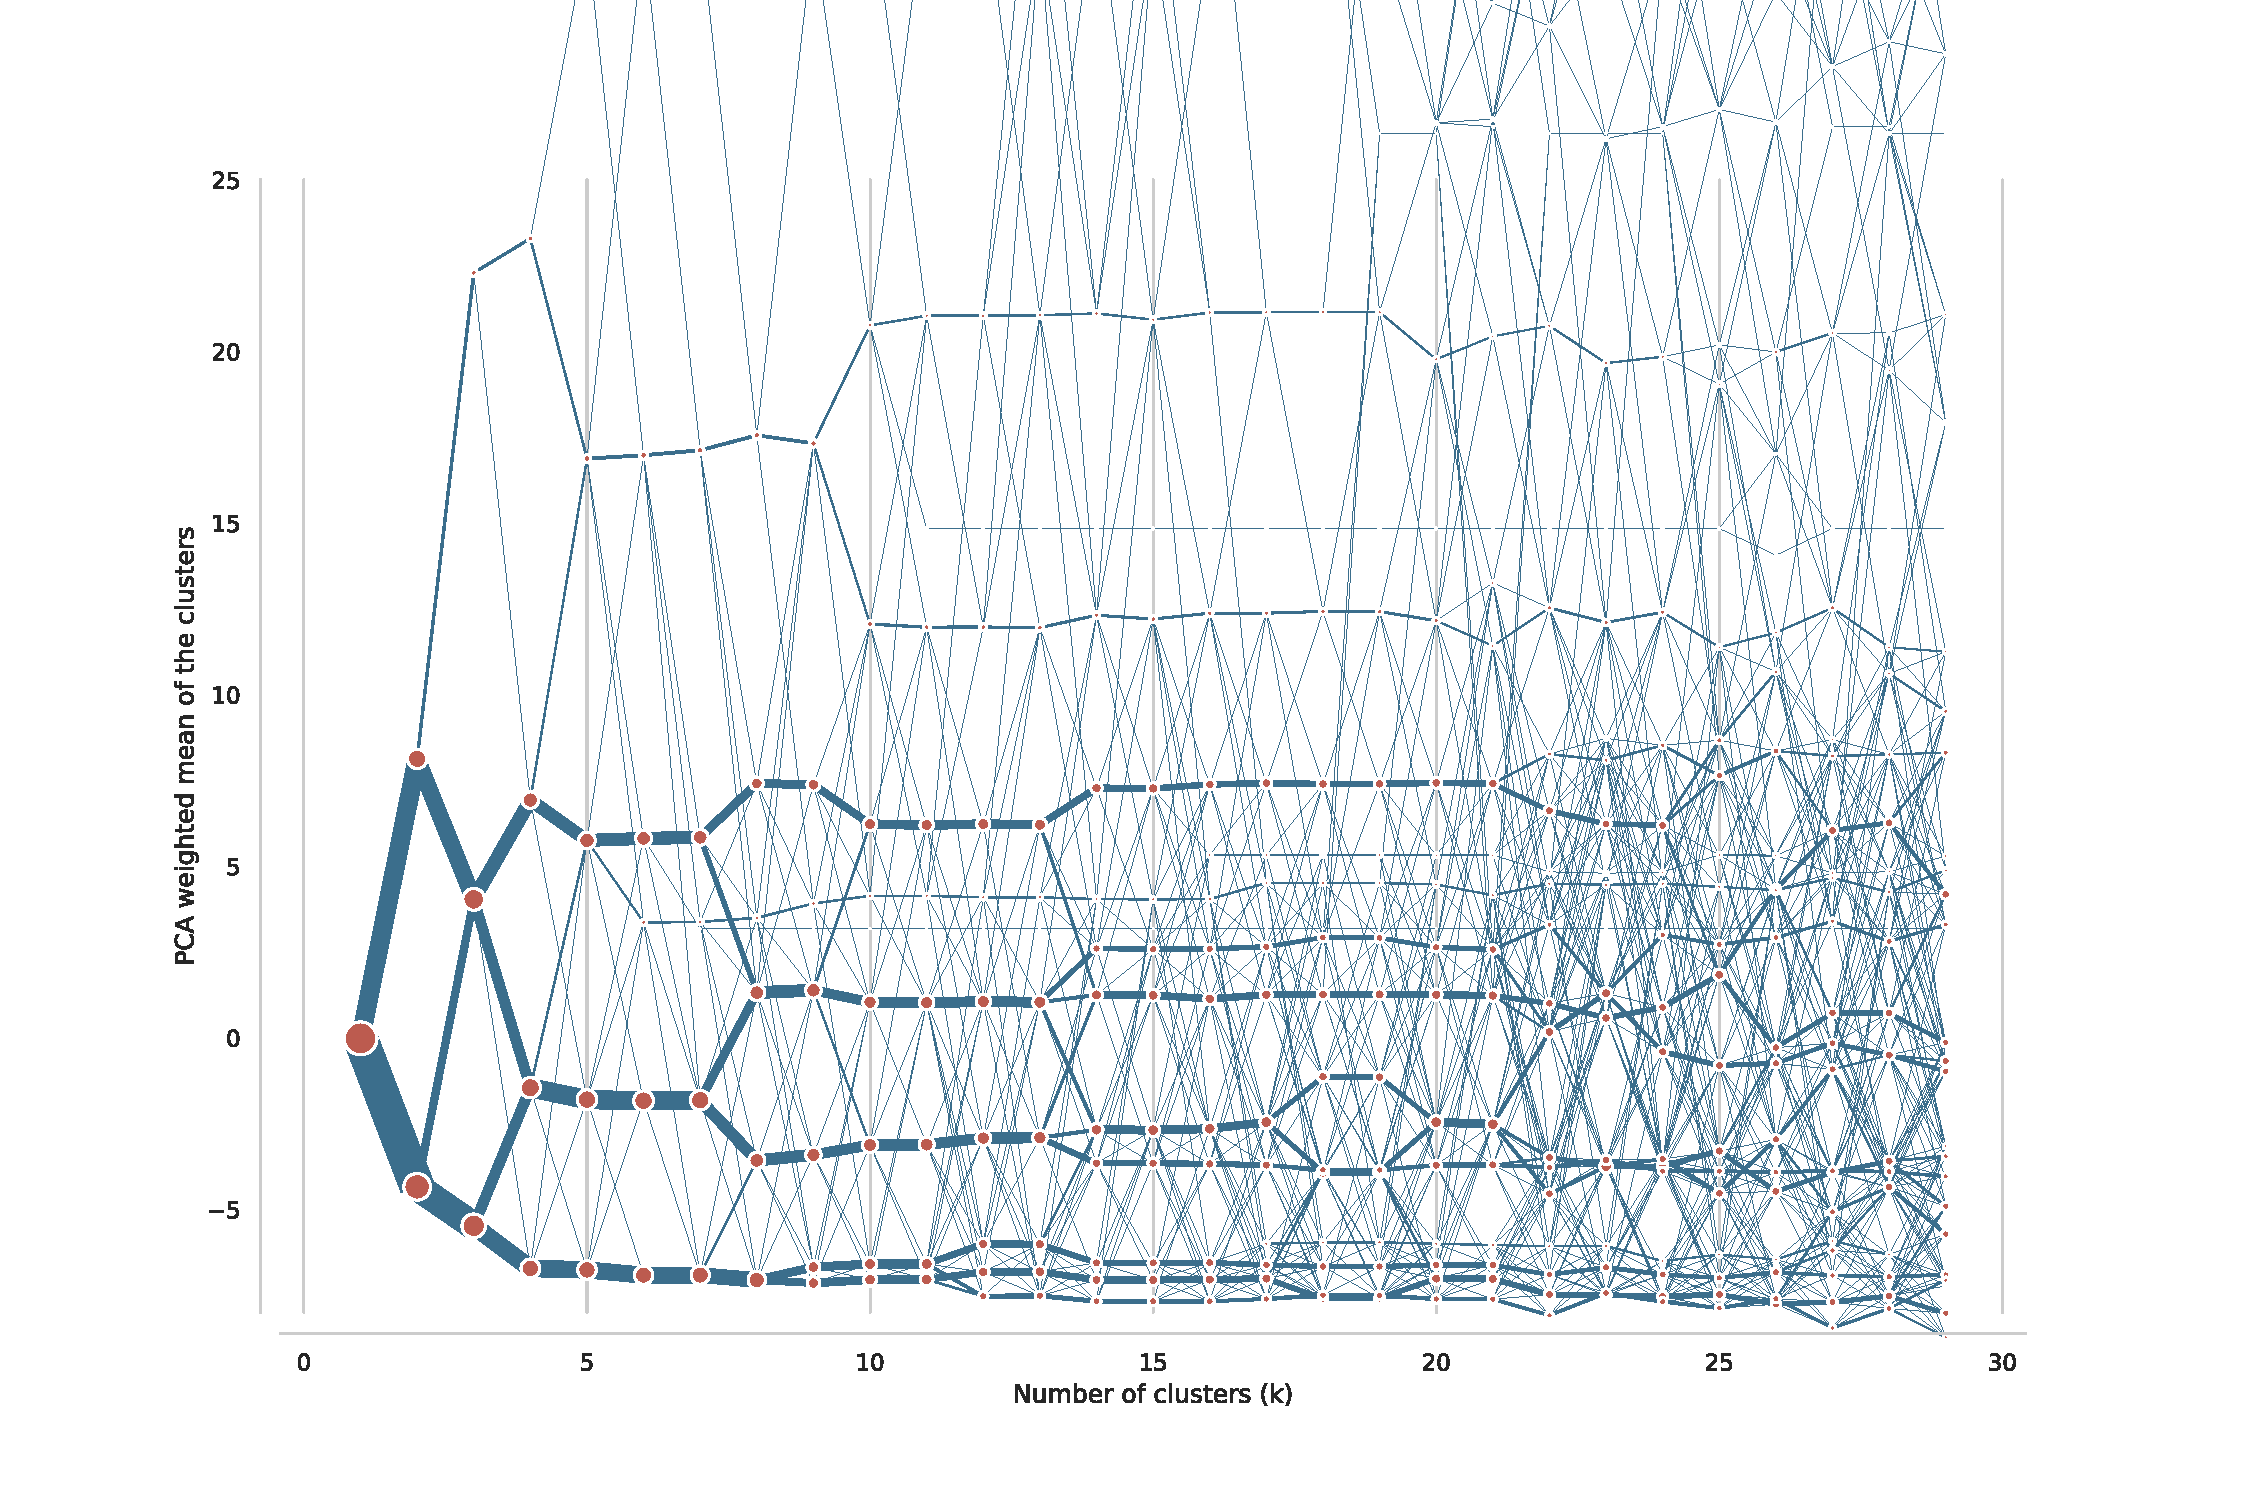
\includegraphics[width=\linewidth]{figures/clustergram_bcn.pdf}
    \caption{Clustergram (truncated along the vertical axis) illustrating the behaviour of dataset in different clustering options. The optimal number of clusters derived using the clustergram is 16.}
    \label{fig:cgram_bcn}
\end{figure}

\begin{figure}
    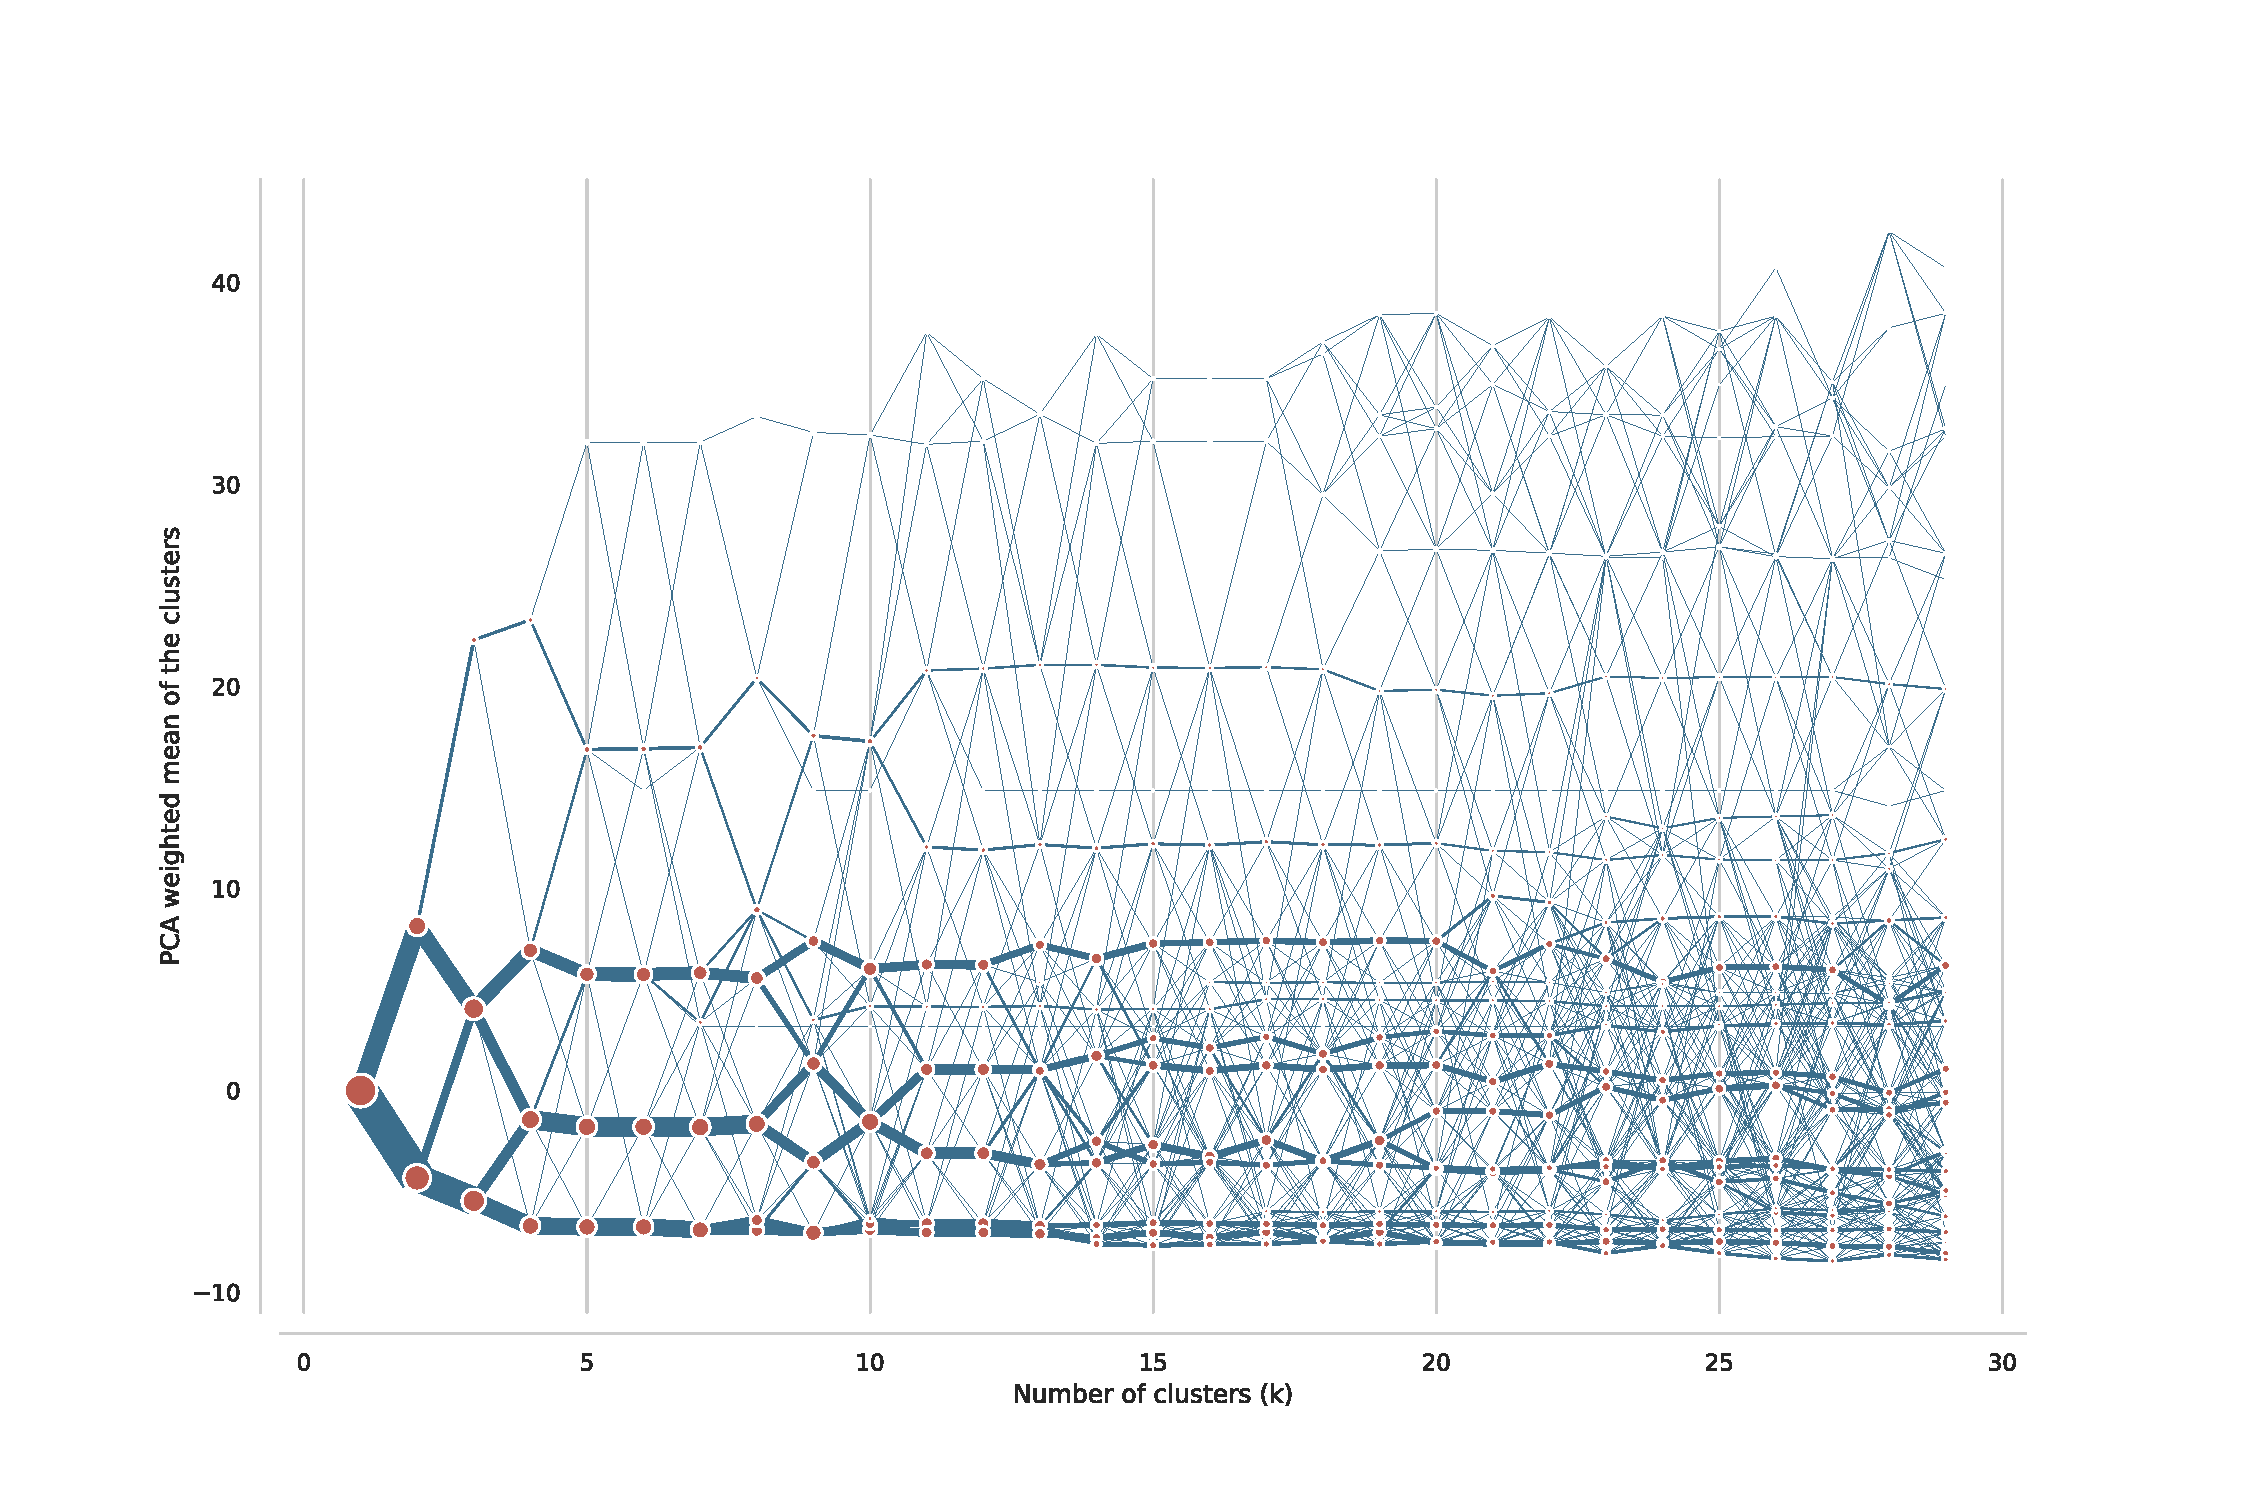
\includegraphics[width=\linewidth]{figures/clustergram_med.pdf}
    \caption{Clustergram (truncated along the vertical axis) illustrating the behaviour of dataset in different clustering options. The optimal number of clusters derived using the clustergram is 19.}
    \label{fig:cgram_med}
\end{figure}

\begin{figure}
    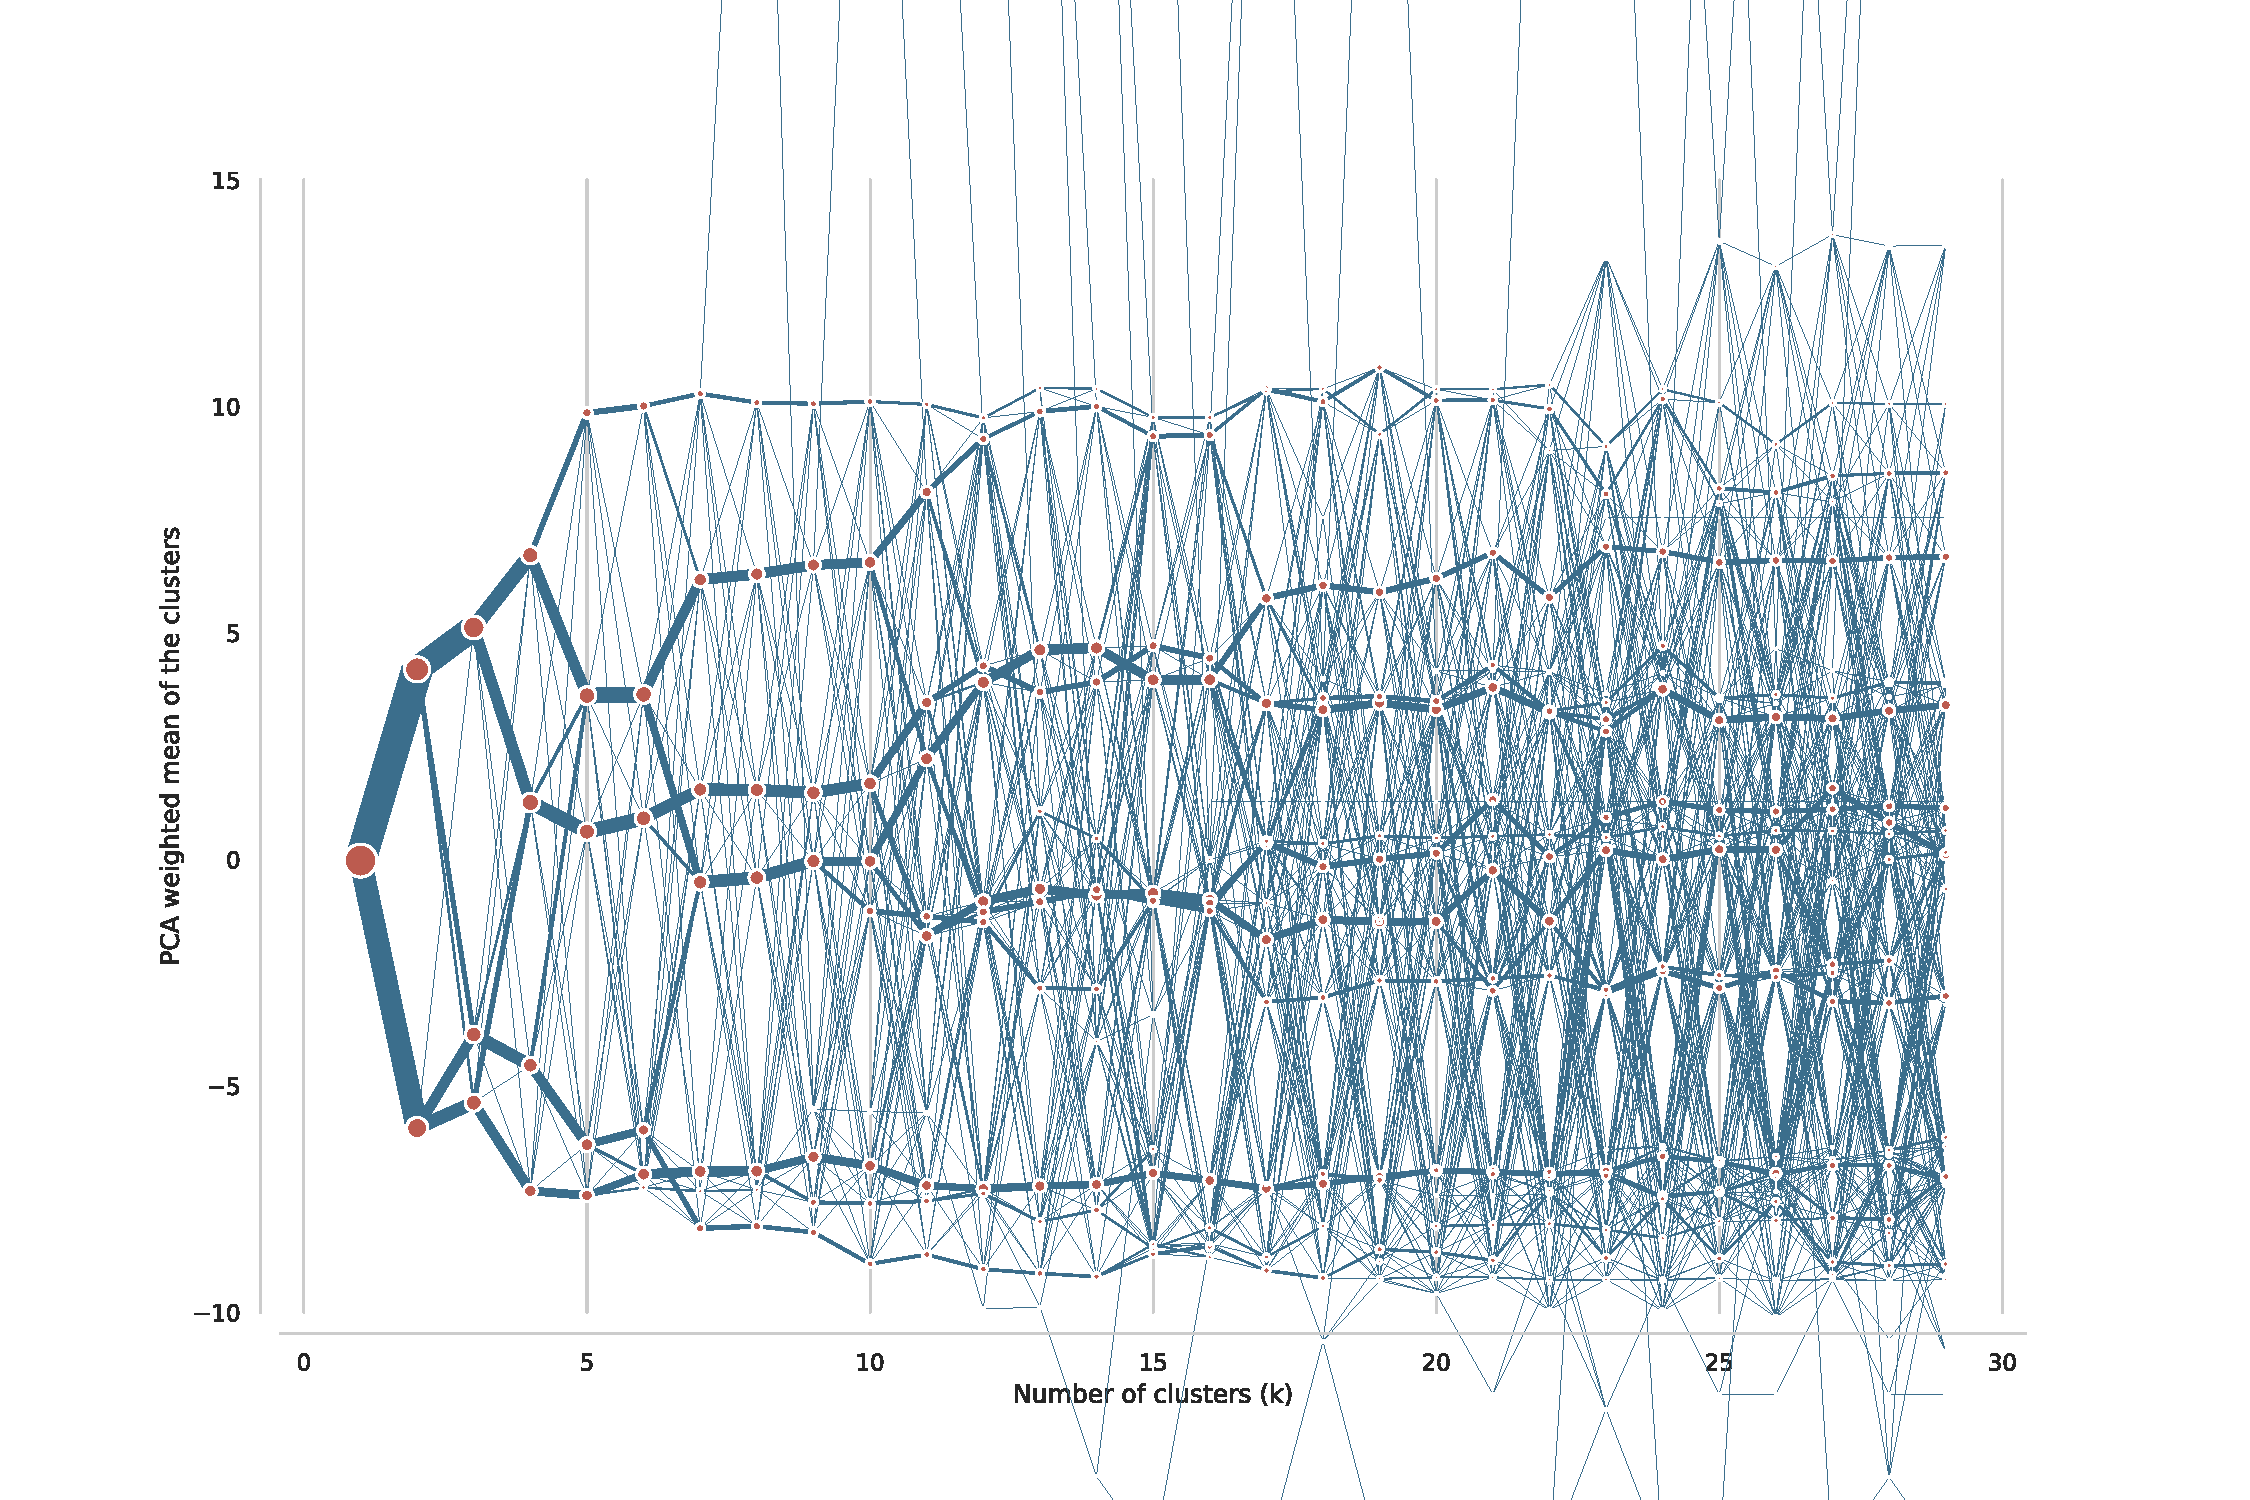
\includegraphics[width=\linewidth]{figures/clustergram_des.pdf}
    \caption{Clustergram (truncated along the vertical axis) illustrating the behaviour of dataset in different clustering options. The optimal number of clusters derived using the clustergram is 17.}
    \label{fig:cgram_des}
\end{figure}

\begin{figure}
    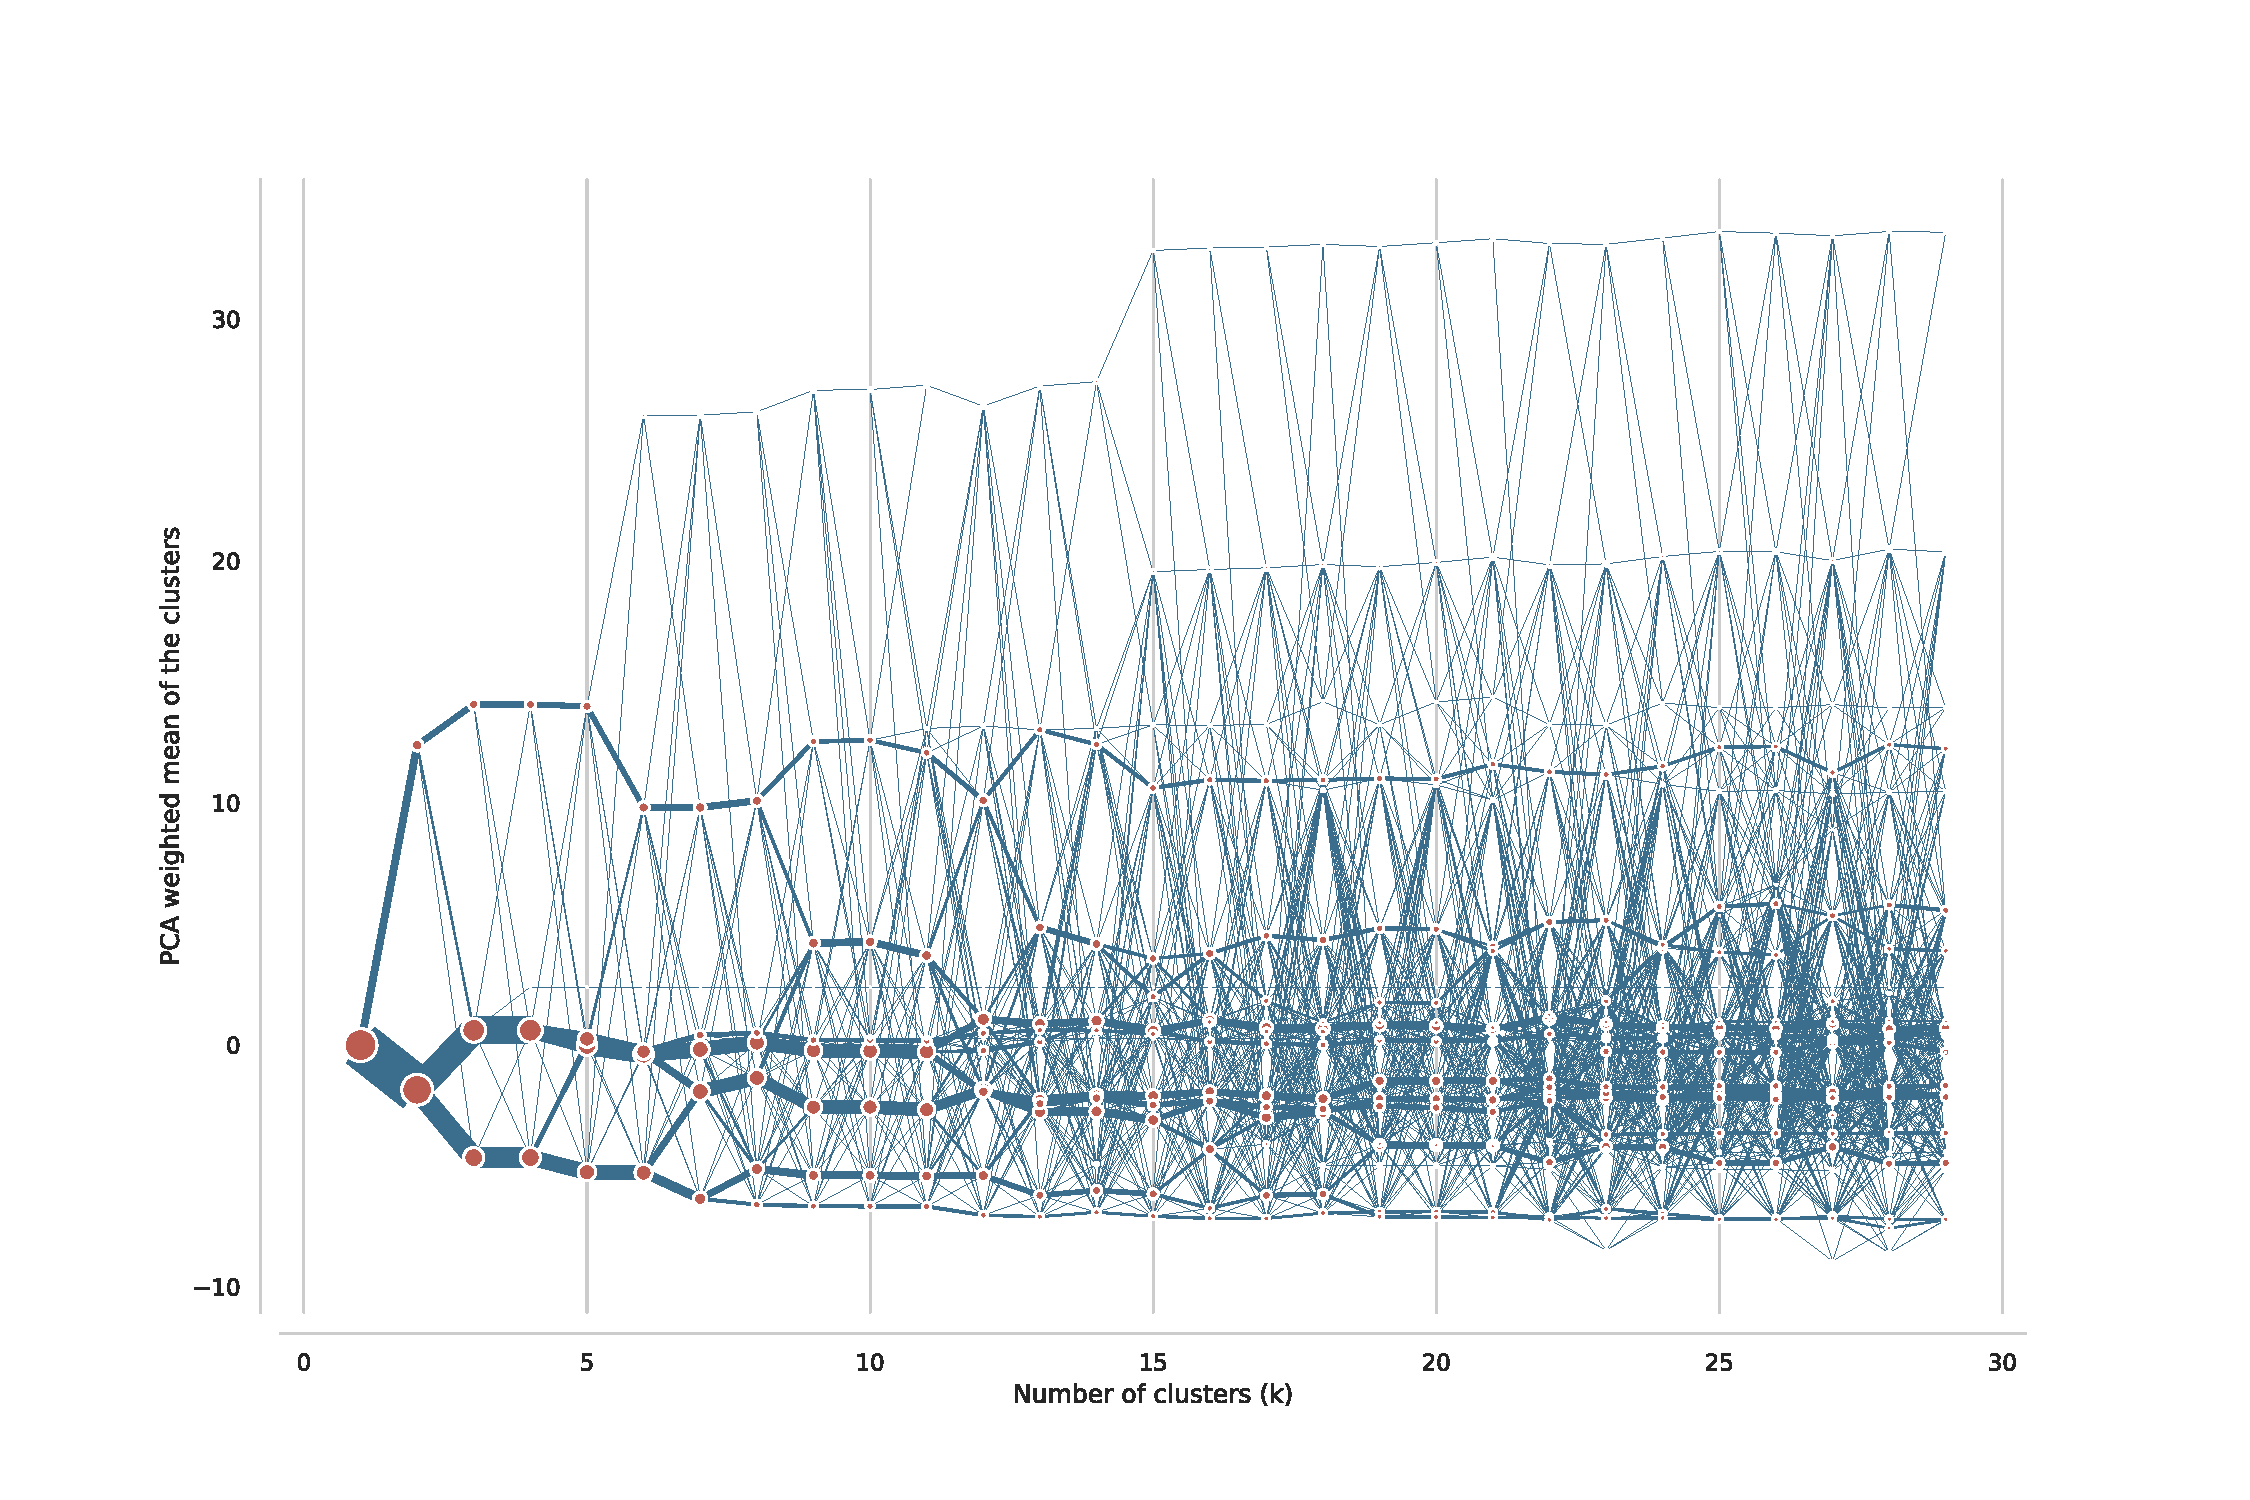
\includegraphics[width=\linewidth]{figures/clustergram_hou.pdf}
    \caption{Clustergram (truncated along the vertical axis) illustrating the behaviour of dataset in different clustering options. The optimal number of clusters derived using the clustergram is 9.}
    \label{fig:cgram_hou}
\end{figure}

\begin{figure}
    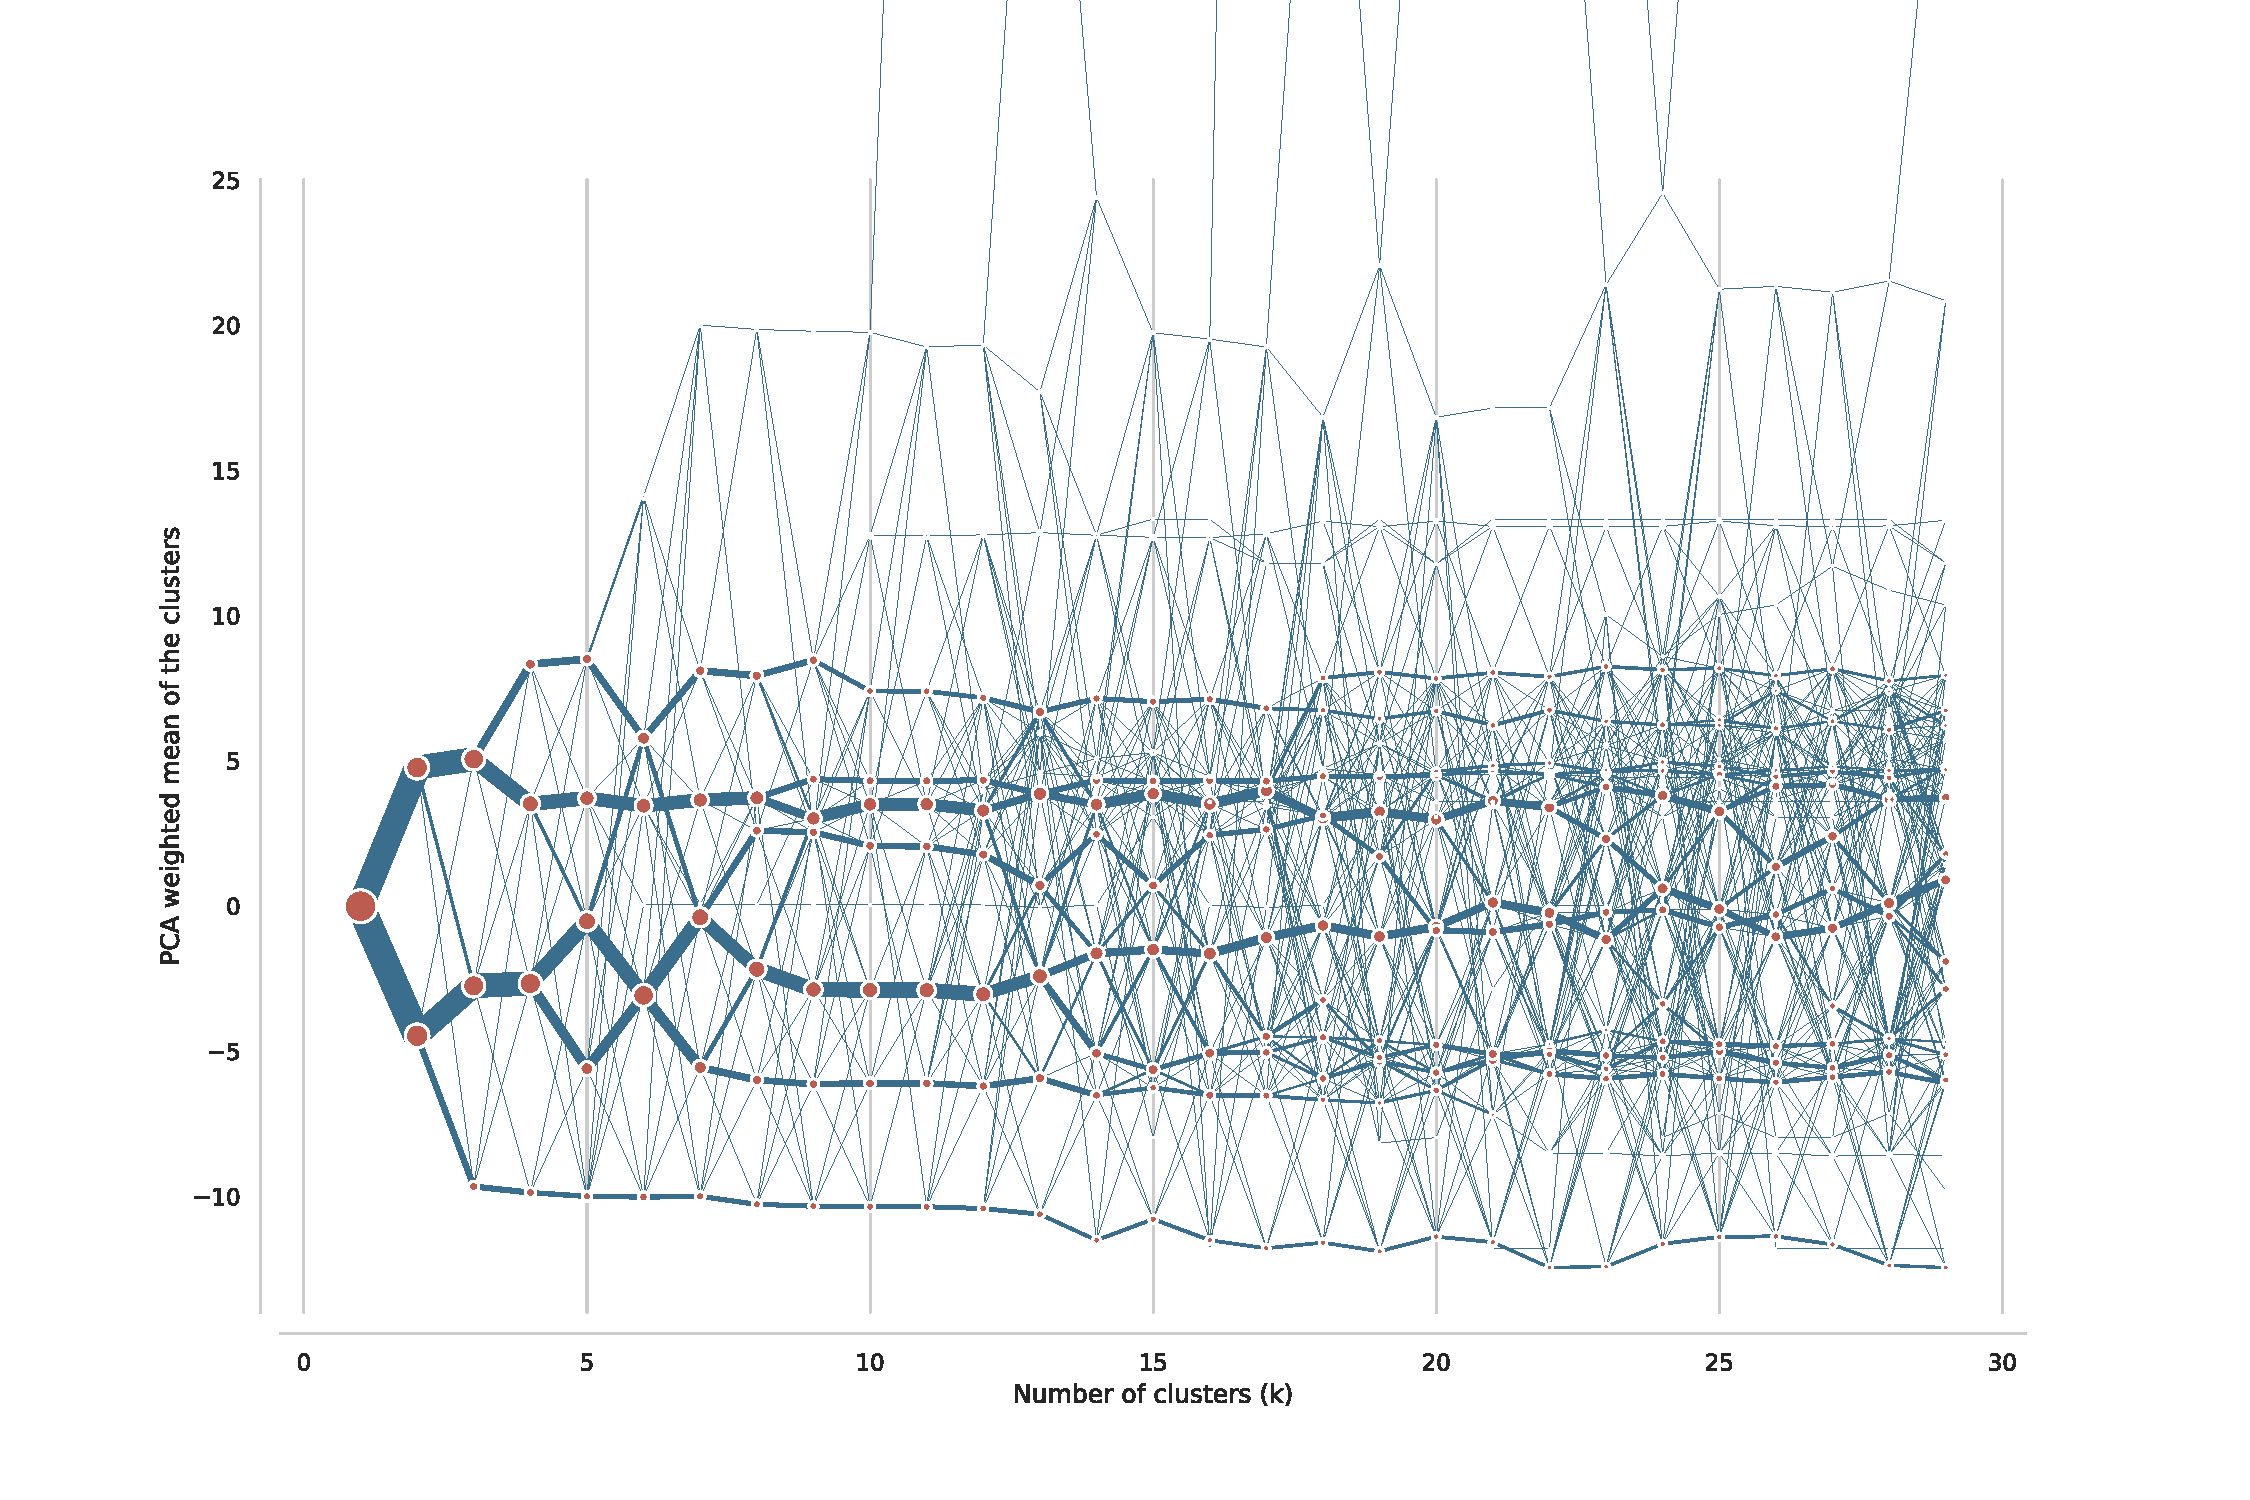
\includegraphics[width=\linewidth]{figures/clustergram_sin.pdf}
    \caption{Clustergram (truncated along the vertical axis) illustrating the behaviour of dataset in different clustering options. The optimal number of clusters derived using the clustergram is 16.}
    \label{fig:cgram_sin}
\end{figure}